\subsection{Seriel kommunikation}

\subsubsection{DevKit8000-PSoC Master}
Til test af denne forbindelsen blev der sendt data fra DevKit8000, ved at skrive ud til den fil i /dev som var forbundet til SPI hardwaren. Herefter blev der
med Logic analyser målt MOSI (udgangen på DevKit8000), CLK(klokken), SS(slave select). Der blev kigget på om de rigtige databits blev skrevet ud
til MOSI, om SS gik lav ved dataoverførelse, og om CLK havde den rigtige clockmode. Efterfølgende blev der også læst fra den samme fil i /dev, og der blev målt
på MISO(Indgangen på DevKit8000).

\subsubsection{PSoC Master - PSoC Slave}
Til test af PSoC-PSoC forbindelsen, blev der tilføjet et UART modul i PSoC creator. Dette gjorde det muligt at skrive de resultater som blev send til PSoC 
enhederne til en terminal på en PC, hvor disse nemt kunne aflæses. Der blev også målt med Logic Analyzer for at teste om de fire forbindelser MISO, MOSI, CLK 
og SS og rigtig ud ligsom i testen mellem DevKit8000 og PSoC Master. På figur xx ses testopstilling for PSoC-PSoC\\

\begin{figure}[H]
	\centerline{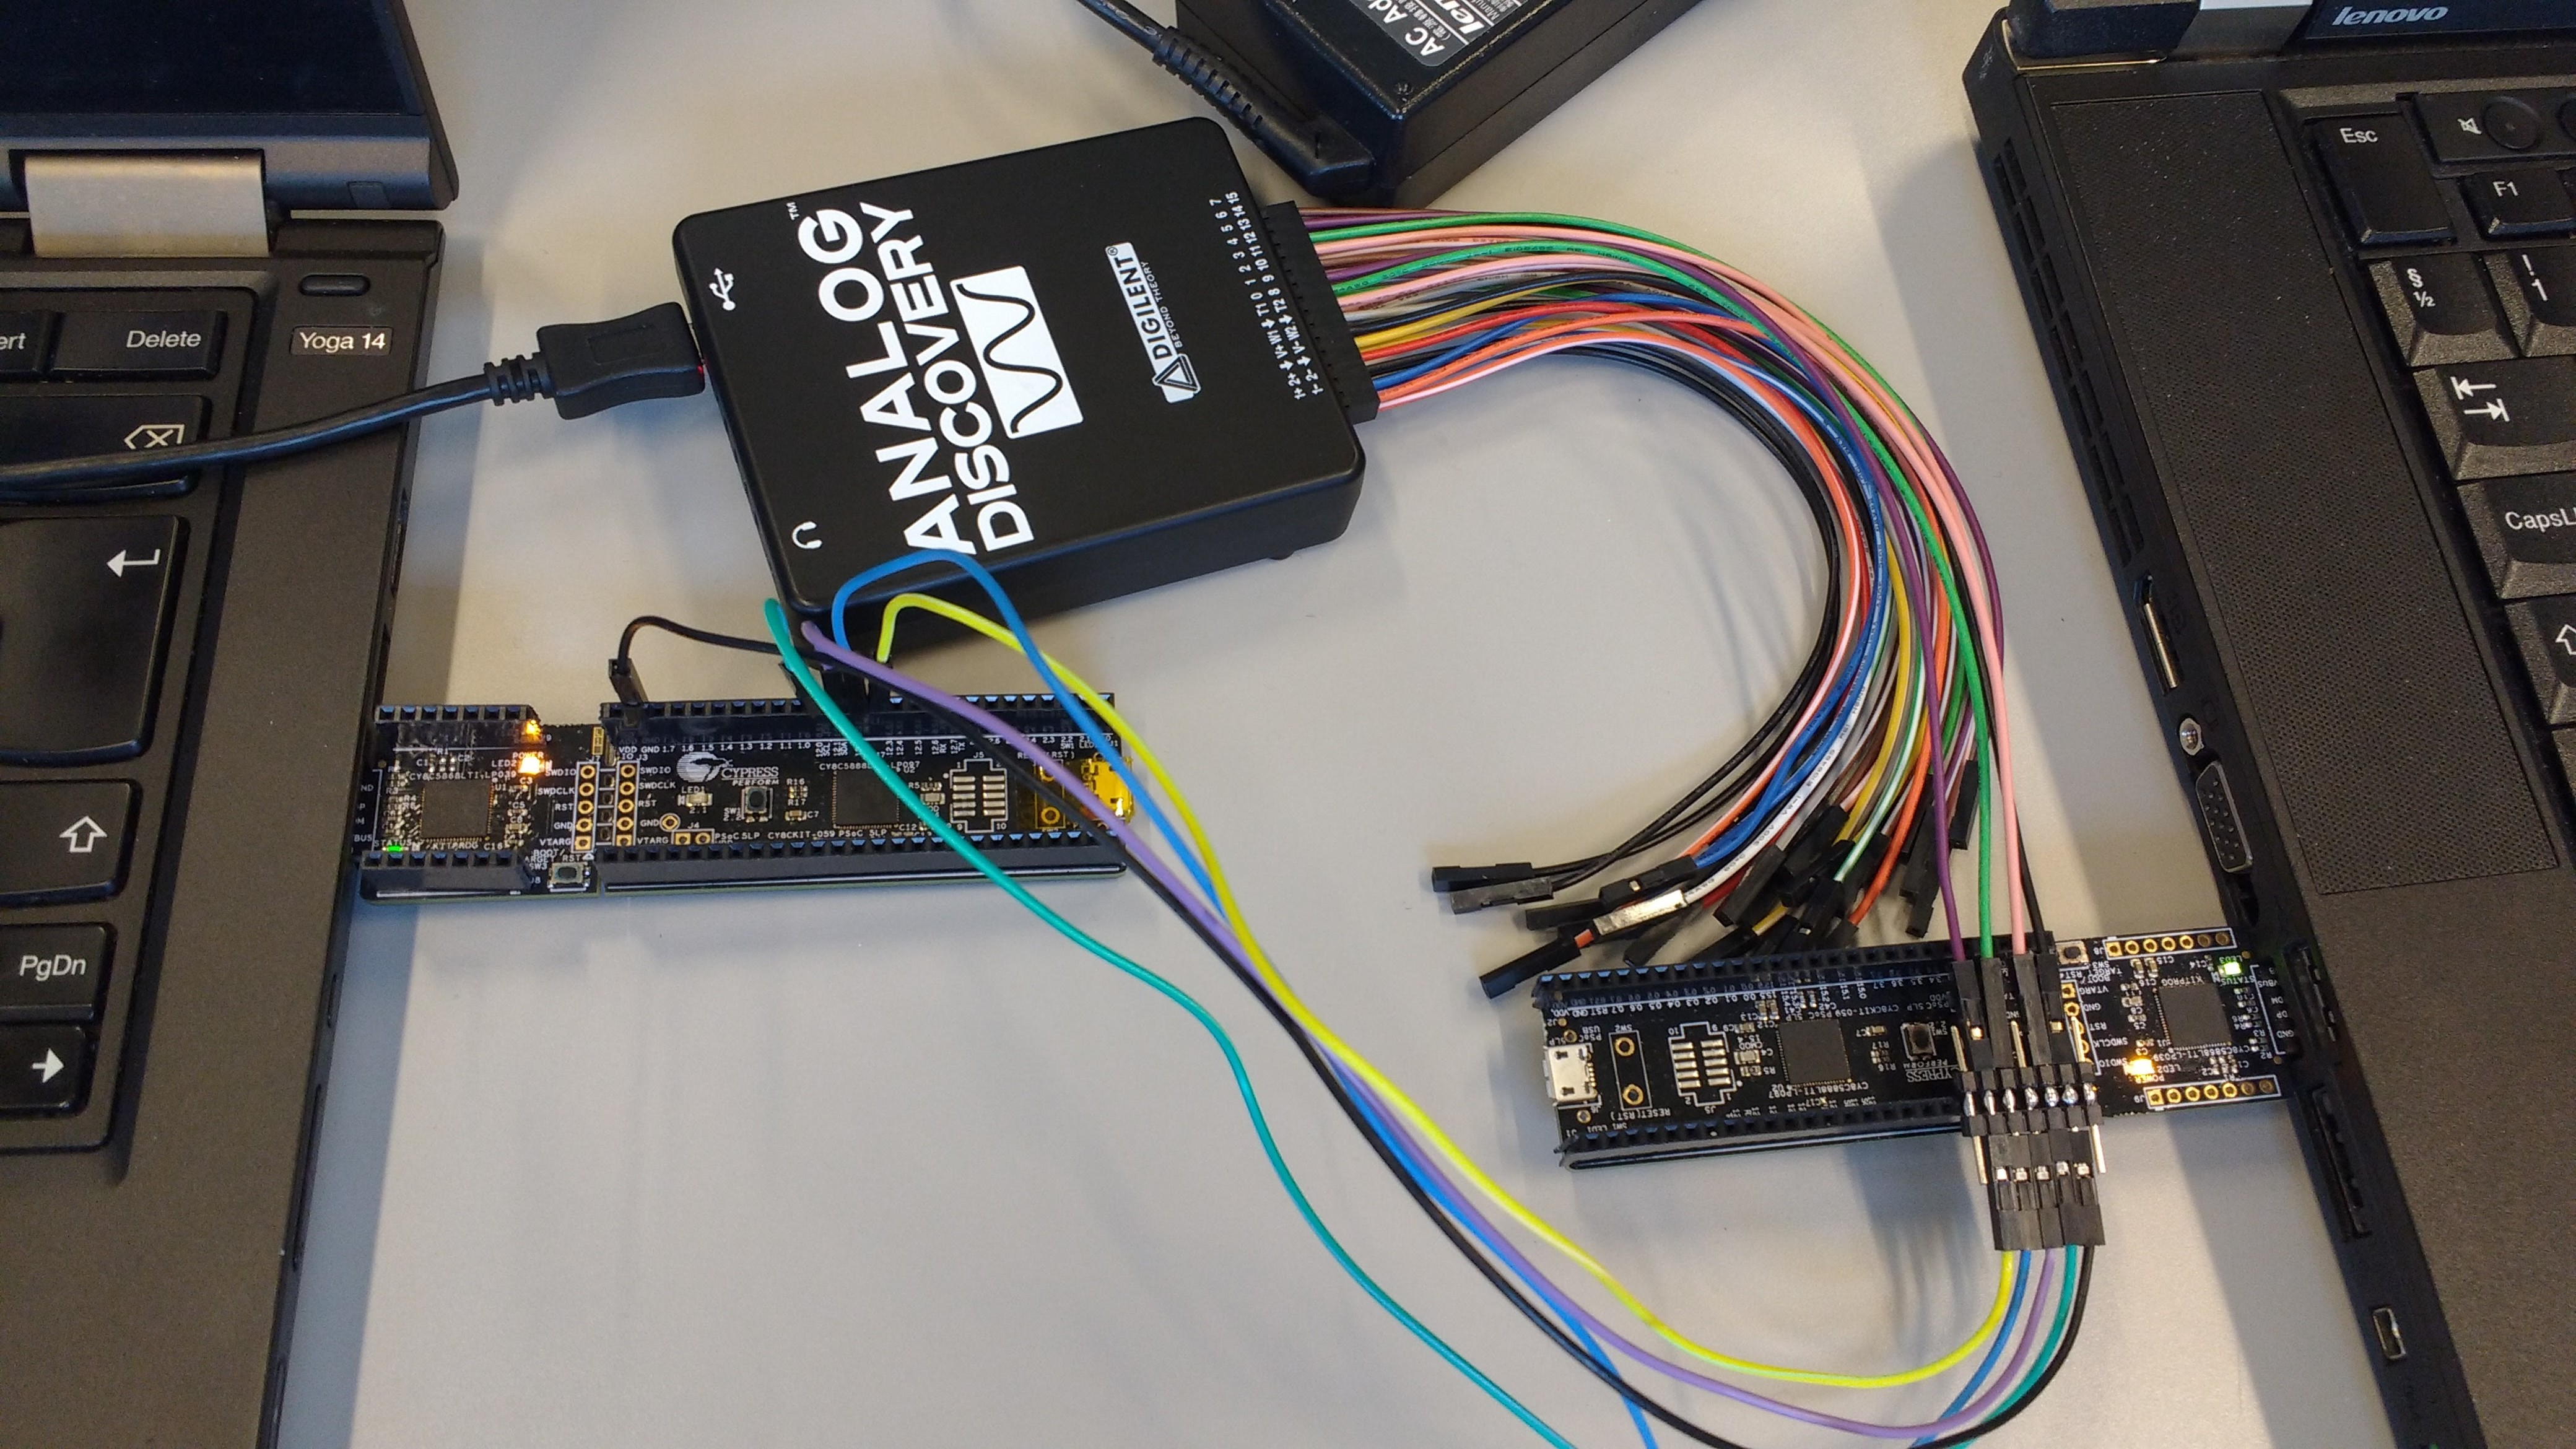
\includegraphics[scale=0.07]{tex/TeImRe/SPI/SPI_testAnalog}}
	\caption{testopstilling for PSoC Master/PSoC Slave forbindelsen}
\end{figure}